\documentclass{IEEEtran}
\usepackage{microtype}
\usepackage{cite}
\usepackage[pdftex]{graphicx}
\usepackage{amsmath}
\usepackage[margin=0.35in]{geometry}
\title{Learning from the Past \\{\large Assessing and Modeling Viral Vaccination in the Face of a Pandemic}}
\author{\small Nicholas Garside\textemdash Mechanical Engineering PhD, 2\textsuperscript{nd} year \\
Arinze Okafor\textemdash Biomedical Engineering PhD, 2\textsuperscript{nd} year \\
 Lucy Chikwetu\textemdash Biomedical Engineering PhD, 3\textsuperscript{rd} year  }
\begin{document}
\twocolumn[
\begin{@twocolumnfalse}
\maketitle
{\huge Background}\\\\
Throughout history, the outbreak of viral infections poses one of the greatest threats to human health and civilization. The occurrence of viral pandemics has, each time, resulted in the loss of thousands to millions of lives, the crippling of global economies and supply chain, and the straining of healthcare systems~\cite{HuremoviA2019}. Vaccination remains one of the most effective long-term instruments to combat these debilitating effects. Despite its extreme importance, societal response to vaccination has not always been optimal and is influenced by several socioeconomic factors~\cite{youngVax}.\\\\
In 2009, an outbreak of a novel influenza A (H1N1 class) virus led to the death of over half a million people. Concerted efforts to tackle this outbreak led to the development of a new H1N1 viral vaccine only seven months after the initial outbreak. Despite this success, societal acceptance and vaccination rates for both the H1N1 virus and seasonal flu remained low~\cite{ravert_fu_zimet_2012}~\cite{cdc}.\\\\ 
Following the path of history, the recent outbreak of the Severe Acute Respiratory Syndrome-Corona Virus 2 (SARS-CoV2) has resulted in the infection of over 30 million people worldwide, while causing the death of over a million people~\cite{jhu}. Despite this unsavory development, societal attitude to the ongoing global vaccination efforts remains less than optimal, with close to half of the US population having negative or pessimistic views~\cite{fisher}. Given this undesired societal attitude, even in the face of the current pandemic, and the importance of vaccination in saving lives and the global economy, it becomes imperative to utilize analytical tools to better understand the factors affecting vaccine acceptance, predict compliance to vaccination advisories, and guide the channeling of resources to maximize rates of vaccination in a bid to save lives.\\\\ 
{\huge Aim of Study}\\\\
We hypothesize that the 2009 H1N1 viral outbreak allows us to learn about COVID-19 in retrospect.  This study aims to harness available datasets from the 2009 pandemic and machine learning approaches in assessing factors affecting an individual's likelihood to get a vaccine. We plan to extrapolate these results to propose recommendations for implementing a future voluntary COVID-19 vaccine.\\\\ 
{\huge Data Description}\\\\
The dataset came from an in-person National 2009 H1N1 Flue Survey conducted by the National Center for Health Statistics (NCHS) and the National Center for Immunization and Respiratory Diseases (NCIRD) in a bid to study the socio-economic effects influencing vaccine compliance. Nearly 40,000 United States citizens participated in the study.  In addition to capturing demographic information, the survey also gauged individuals' opinions on H1N1 or seasonal flu vaccine effectiveness, solicited behavioral tendencies, and asked participants whether or not their doctor recommended an H1N1 or flu vaccine.  The dataset has 35 features, a respondent ID, and two target variables\textemdash \textbf{\emph{h1n1\textunderscore vaccine}} abd \textbf{\emph{seasonal\textunderscore vaccine}}. Both target variables are dichotomous variables indicating whether or not an individual received a vaccine. The data includes a healthy mix of nominal variables, ordinal variables, and dichotomous features such as gender and marital status.  Table 1. shows the summary of statistics for available features and the output.\\\\
{\huge Missing Values}\\\\ 
Within the training dataset, there were 13201 observations (49.4$\%$) with missing values in a total of 23 of the 35 predictor variables. Fig 2. is the visual representation of our missing values. Without a doubt, health insurance had the most missing values. We also recognize some unique patterns that facilitate smooth imputation. Those who did not fill out their opinions on particular issues tended not to fill out most of the opinion section. Children under six months old also missed information about whether or not they were healthcare workers, had health insurance, or had chronic medical conditions, and data imputation for such cases was easy. Fig 3. and Fig. 4 support the validity of those special cases. We also made intelligent inferences to impute missing values, for example, if an individual's employment status was listed as \emph{Not in Labor Force} or \emph{Unemployed} and they had no occupation, we created a new occupation and employent indusry factor called \emph{Unemployed} and we would list the individual in that category.
\end{@twocolumnfalse}
]


\twocolumn[
\begin{@twocolumnfalse}


\begin{center}
{\small
\begin{tabular}{p{8cm} p{0.5cm} p{10cm}}
{\small Summary statistics for ordinal variables } & & {\small Summary statistics for dichotomous variables }\\ 

\begin{tabular}{| l |c|c|c|c|}
\hline 
& \textbf{min} & \textbf{mean} & \textbf{median} & \textbf{max} \\
\hline 
h1n1\textunderscore concern & 0 & 1.618 & 2 & 3\\
\hline
h1n1\textunderscore knowledge & 0 & 1.263 & 1 & 2 \\
\hline 
opinion\textunderscore h1n1\textunderscore vacc\textunderscore effective & 1 & 3.851 & 4 & 5\\
\hline 
opinion\textunderscore h1n1\textunderscore risk & 1 & 2.343 & 2 & 5\\
\hline 
opinion\textunderscore h1n1\textunderscore sick\textunderscore from\textunderscore vacc & 1 & 2.358 & 2 & 5\\
\hline
opinion\textunderscore seas\textunderscore vacc\textunderscore effective & 1 & 4.026 & 4 & 5\\
\hline 
opinion\textunderscore seas\textunderscore seas\textunderscore risk & 1 & 2.719 & 2 & 5\\
\hline 
opinion\textunderscore seas\textunderscore sick\textunderscore from\textunderscore vacc & 1 & 2.118 & 2 & 5\\
\hline
household\textunderscore adults & 0 & 0.887 & 1 & 3\\
\hline 
household\textunderscore children & 0 & 0.535 & 0 & 3\\
\hline 
\multicolumn{4}{l}{}\\
\multicolumn{4}{l}{\textbf{List of nominal variables}}\\
\hline
\multicolumn{4}{l}{age\textunderscore group, education, race, sex, income\textunderscore poverty}\\
\multicolumn{4}{l}{marital\textunderscore status, rent\textunderscore or\textunderscore own, employment\textunderscore status}\\
\multicolumn{4}{l}{hhs\textunderscore geo\textunderscore region, census\textunderscore msa, employment\textunderscore industry}\\
\multicolumn{4}{l}{employment\textunderscore occupation}
\end{tabular} &  &% end of first table 


\begin{tabular}{| l |c|c|c|c|} %second table 
\hline 
& \textbf{min} & \textbf{mean} & \textbf{median} & \textbf{max} \\
\hline 
behavioral\textunderscore antiviral\textunderscore meds & 0 & 0.049 & 0 & 1\\
\hline
behavioral\textunderscore avoidance & 0 & 0.726 & 1 & 1\\
\hline 
behavioral\textunderscore face\textunderscore mask & 0 & 0.069 & 0 & 1\\
\hline 
behavioral\textunderscore wash\textunderscore hands & 0 & 0.826 & 1 & 1\\
\hline 
behavioral\textunderscore large\textunderscore gatherings & 0 & 0.359 & 0 & 1\\
\hline
behavioral\textunderscore outside\textunderscore home & 0 & 0.337 & 0 & 1\\
\hline 
behavioral\textunderscore touch\textunderscore face & 0 & 0.677 & 1 & 1\\
\hline 
doctor\textunderscore recc\textunderscore h1n1 & 0 & 0.220 & 0 & 1\\
\hline 
doctor\textunderscore recc\textunderscore seasonal & 0 & 0.330 & 0 & 1\\
\hline 
chronic\textunderscore med\textunderscore condition & 0 & 0.283 & 0 & 1\\
\hline 
child\textunderscore under\textunderscore 6\textunderscore months & 0 & 0.083 & 0 & 1\\
\hline
health\textunderscore worker & 0 & 0.1122 & 0 & 1\\
\hline
health\textunderscore insurance & 0 & 0.880 & 1 & 1\\
\hline
seasonal\textunderscore vaccine & 0 & 0.466 & 0 & 1\\
\hline
h1n1\textunderscore vaccine & 0 & 0.213 & 0 & 1\\
\hline
\multicolumn{4}{l}{}\\
\end{tabular}\\
& & \\
\multicolumn{3}{c}{Table 1: Summary of statistics of all variables (including the output)}\\
\end{tabular}%outer table 
}
\end{center}
{\huge Distributions}\\
We plotted stacked bar graphs to show each feature's relationship with the target variable\textemdash no strong associations where identified for the H1N1 vaccine, but interesting associations were identified for seasonal flu vaccine. H1N1 vaccine had a mean of 0.2125 and seasonal flu vaccine had 0.4656, and this could have contributed to the disparity we observed.  Fig. 1 shows the plots for each feature's relationship with the seasonal flu vaccine. \\\\
{\huge Preliminary Relationships Between Features}\\\\
The team did a preliminary analysis of the ordinal and binary features' correlations using Spearman?s ranking method. Results from this analysis have are shown in Fig. 5, with only significant correlations being displayed. This analysis briefly revealed a significant positive correlation between the features: concern about the H1N1 virus, positive opinions on the vaccine, and age; and vaccine compliance (p$<$0.05). Also, older people seemed to have higher vaccination compliance (p$<$0.05), and people tend to comply more when their doctors recommend the vaccine (p$<$0.05). The relationship between the nominal variables and the outcome variables was accessed using the Chisquare test for statistical independence. This revealed that, of all six nominal variables (employment occupation, employment industry, employment occupation, region of residence as defined by the U.S. Dept. of Health and Human Services, region of residence by the metropolitan statistical areas and race), compliance with H1N1 vaccination were not independent of the respondent?s region of residence defined by the metropolitan statistical areas (X-squared = 0.11411 , P=0.95). This was not the case for compliance with seasonal vaccination. However, the interpretation of this is limited as the exact metropolitan statistical areas have been deidentified, making it difficult to know which areas were compliant and which were not.\\\\
{\huge Possible Modeling Approaches}\\\\
This dataset is part of an online competition hosted by drivendata.org~\cite{drivendata}. The competition's organizers split the dataset into two halves--one for training and another for testing. Label values (h1n1\textunderscore vaccine and seasonal\textunderscore vaccine) were only provided for the training data with a training data sample size of 26,707. The test dataset labels were withheld to facilitate the unbiased evaluation of model performance for the competition. We plan to further split the training set provided into training, validation, and testing datasets in order to enable model training, prevent model overfitting and enable model evaluation. We will split the data set into three groups using a split ratio of 60:20:20 for training, validation, and testing, respectively. 
To gain some insight into the fundamental linear and non-linear relationships between predictors and our outcome variable, we will explore less flexible but interpretable modeling approaches. Per our study goals and for the competition, we aim to develop a predictive model focusing on maximizing prediction accuracy. For this purpose, we will explore highly flexible approaches such as some tree-based methods (e.g., random forest, XGBoost), neural network-based methods (e.g., Multi-Layered Perceptron). Spanning the degree of model flexibility is a major goal, as we strive to both intuitively understand influencing factors and accurately predict outcomes as we apply our predictions to the real-world problem.\\\\ 
{\huge Conclusion}\\\\
This project aims to answer the currently relevant question: What are the leading predictors of vaccination, and to what extent can we predict novel disease vaccination rates from these features? This question is becoming increasingly relevant as COVID-19 is nearing vaccine completion, for the answer could help guide public vaccination efforts in the future. 
\end{@twocolumnfalse}
]

\onecolumn{
\begin{center}
\begin{tabular}{p{8cm}p{8cm}}
\multicolumn{2}{c}{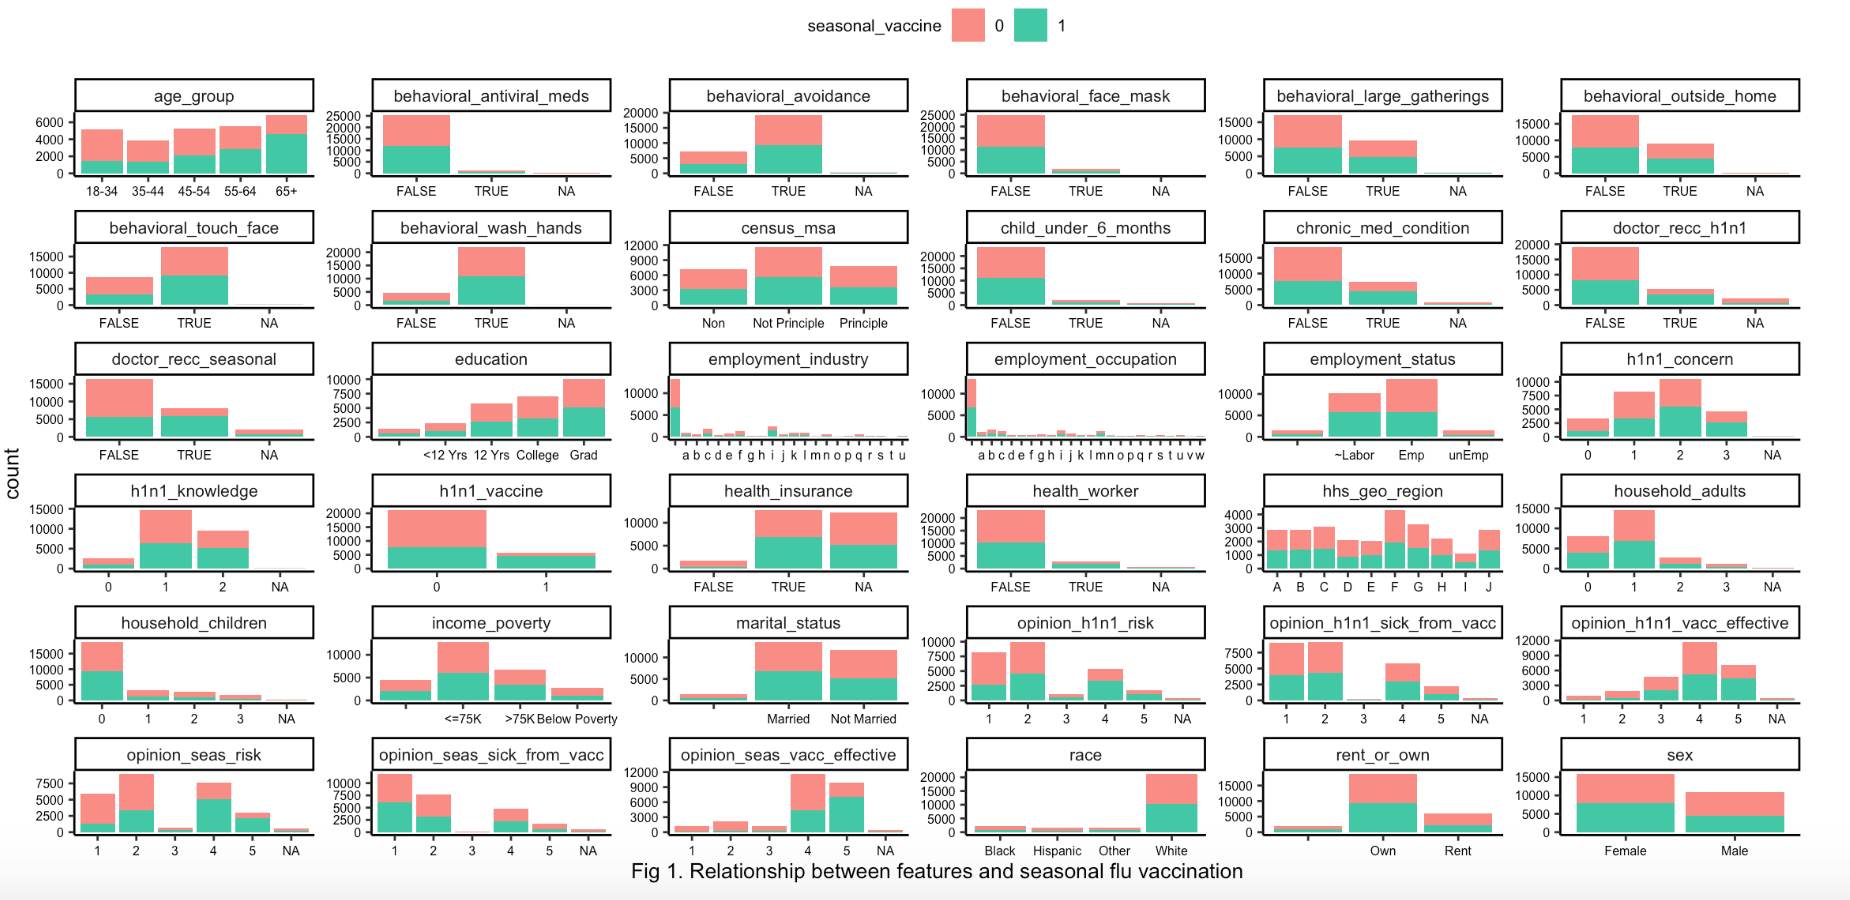
\includegraphics[scale=0.55]{relationships}}\\
\multicolumn{2}{c}{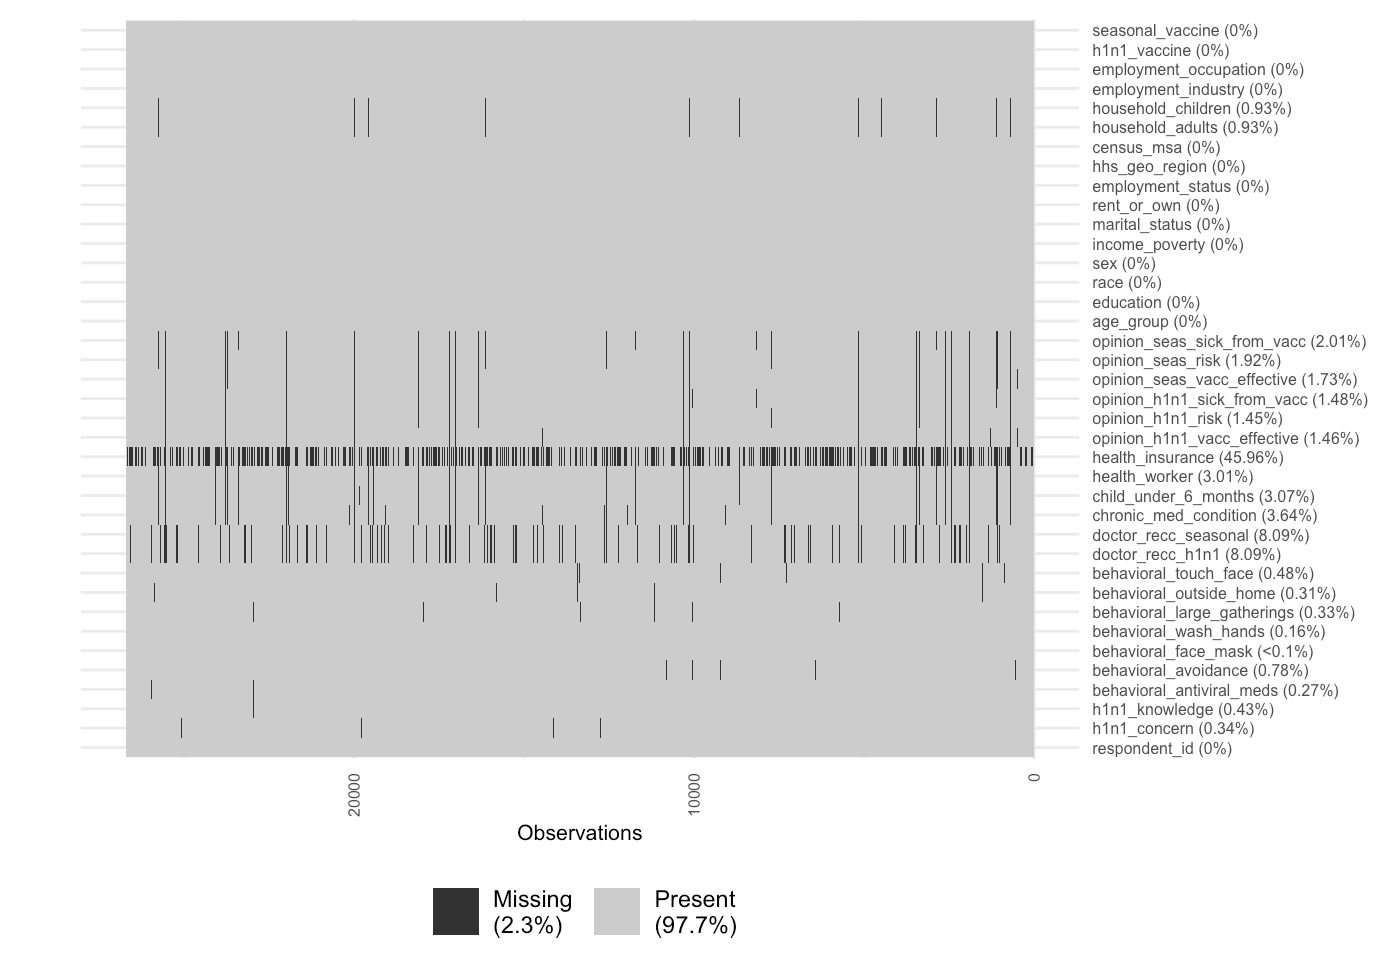
\includegraphics[scale=0.55]{missingnessMap}}\\
\multicolumn{2}{c}{Fig 2. Visual representation of missing values}\\
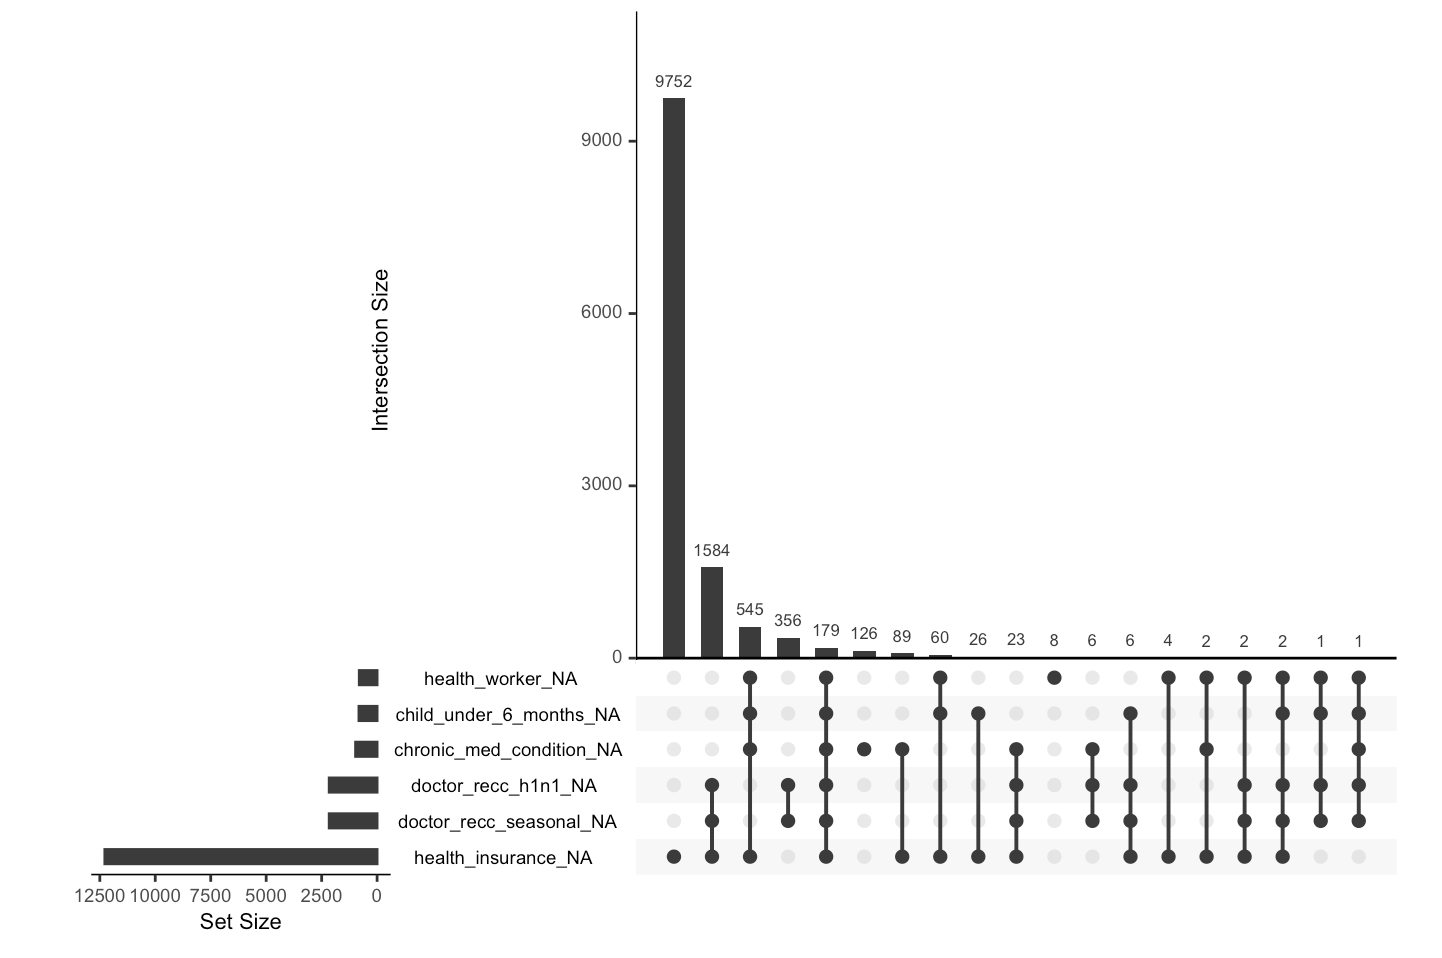
\includegraphics[width=0.53\columnwidth]{children} & 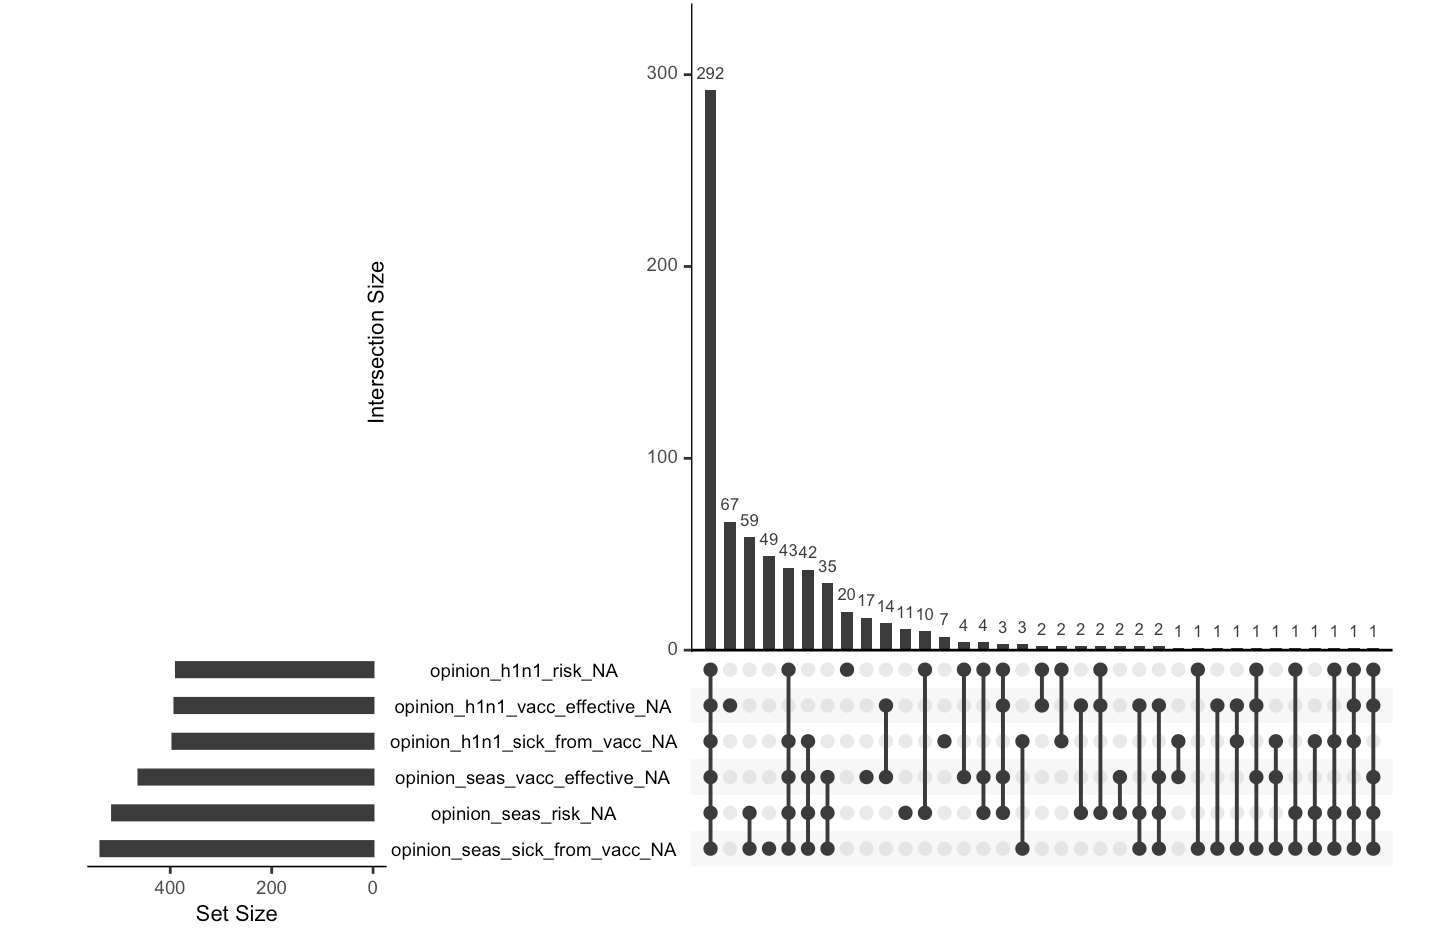
\includegraphics[width=0.53\columnwidth]{opinions}\\
\multicolumn{2}{c}{Fig 3. \hspace{8.5cm} Fig 4.}\\
\end{tabular}
\end{center}
}
\clearpage
\onecolumn{
\begin{center}
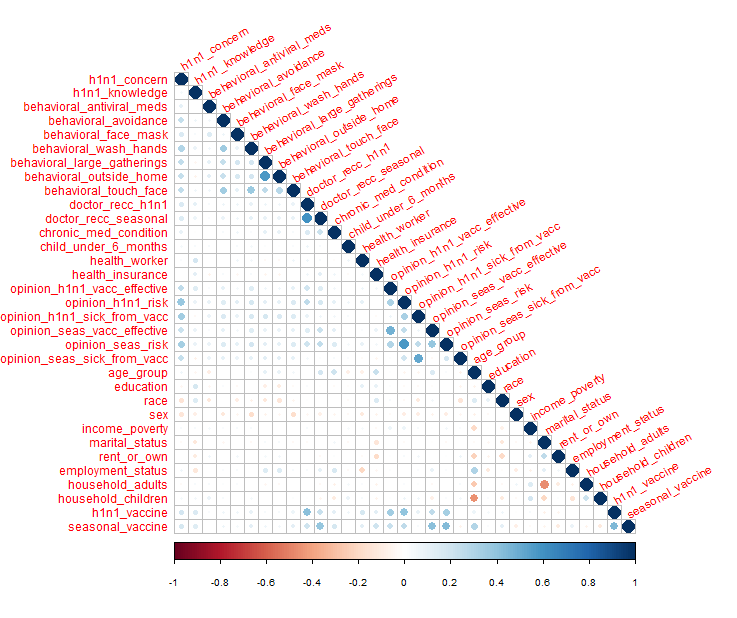
\includegraphics[width=0.6\columnwidth]{corr}\\
Fig. 5 Correlation plot for FluShot features
\end{center}
\bibliographystyle{plain}
\bibliography{proposal_bib}
}
\end{document}